% Prof. Dr. Ausberto S. Castro Vera
% UENF - CCT - LCMAT - Curso de Ci\^{e}ncia da Computa\c{c}\~{a}o
% Campos, RJ,  2021
% Disciplina: Paradigmas de Linguagens de Programa\c{c}\~{a}o
% 



\chapter{ Introdu\c{c}\~{a}o}

Julia é, acima de tudo, uma linguagem ambiciosa. 
Surgiu com o objetivo de solucionar um problema central na computação numérica. O chamado "problema das duas linguagens" se refere ao fato de muitos cientistas, engenheiros e matemáticos usarem uma linguagem flexível e amigável como Python, R, ou Matlab, que os permitia focar no problema sendo investigado ao invés de detalhes de implementação computacional. Porém, logo em seguida ser necessário desenvolver uma nova implementação em linguagem performática como C para de fato computar os dados, pois do contrário enfrentariam um tempo de processamento ordens de grandeza maior e portanto muitas vezes impeditivo. \cite{Lauwens2019}

Mas a ambição de seus criadores, em suas próprias palavras, foi além:

\begin{quote}
   Queremos uma linguagem open source com uma licença liberal. Queremos a velocidade de C com o dinamismo de Ruby. Uma linguagem homoiconica com macros verdadeiras como Lisp, mas com notação matemática obvia e familiar como Matlab. Queremos algo tão geral quanto Python, tão fácil para estatística quanto R, tão natural para processamento de strings quanto Perl, tão poderoso para algebra linear quanto Matlab e tão bom como cola de programas quanto shell. Algo estupidamente simples de aprender, e ainda assim deixe o mais sério dos hackers satisfeito. Queremos algo interativo e que seja compilado. 
   
   Mencionamos que deve ser tão rápida quanto C? 
   \href{https://julialang.org/blog/2012/02/why-we-created-julia/}{[Why We Created Julia, 2012]}
   
   
\end{quote}

Assim foi lançada em 2012 uma linguagem gratuita, de código aberto, alta performance, tipagem dinâmica e paradigma multimétodos que permite expressar procedural, funcional, metaprogramação e orientação a objetos. Com suporte nativo e de alto nível ao paralelismo, alta integração com as extensas bibliotecas já disponíveis para as linguagens que a inspiraram, variáveis unicode com sintaxe de LaTex permitindo letras gregas, subscritos e decoradores, especialmente pensada na computação numérica mas plenamente geral e sim, praticamente tão rápida quanto C. \cite{Lobianco2019,Bezanson2017}

 Nesse trabalho temos uma breve introdução a linguagem Julia, sua história, principais aplicações, sintaxe e ecossistema. 


% Entretanto devido as limitações de tempo foi necessário uma abordagem breve, e voltada a pessoas que já tenham certa familiaridade com programação, entretato podemos recomendar para os iniciantes o livro tal, no qual abordará pontos que não foram considerados aqui.



\newpage
\section{Aspectos históricos da linguagem Julia}

\begin{figure}[H]
   \begin{center}
       \caption{Criadores da linguagem Julia} \label{criadores}
       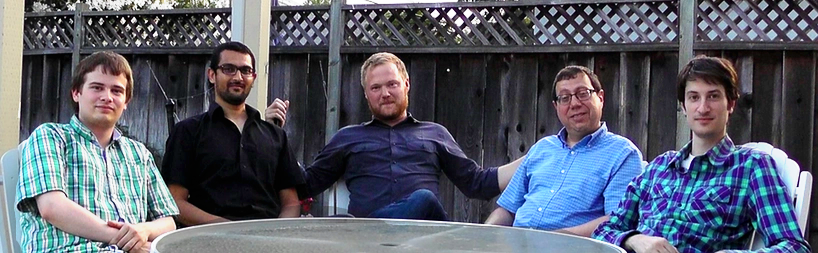
\includegraphics[width=12cm]{creators.png} \\
       {\tiny \sf Fonte: Julia Computing}
   \end{center}
  \end{figure}

Na Fig.\ref{criadores} vemos seus criadores da esquerda para a direita: Keno Fischer, Viral Shah, Stefan Karpinski, Alan Edelman, e Jeff Bezanson.
\newline

Assim como outras linguagens e construtos computacionais, muito de sua história tem pouco registro formal sendo a maior fonte seu site, blog e documentação oficiais, além de palestras em eventos técnicos e artigos jornalísticos, o que torna mais difícil uma recontrução histórica precisa, não obstante, ressaltaremos os principais aspectos à seguir: 
%baseados em: (site julia) 
\begin{itemize}
   \item O nome Julia não tem nenhum significado, foi apenas um nome sugerido por um amigo de Benzanson que os criadores acharam bonito. \footnote{https://docs.julialang.org/en/v1/manual/faq/}
   \item O projeto da linguagem começou em 2009.
   \item Em \href{https://julialang.org/blog/2012/02/why-we-created-julia/}{2012} foi lançada para a comunidade open source. Segundo os criadores com 90\% das características que visionaram, inclusive inicialmente chamaram de Julia 1.0, mas posteriormente adiaram esse marco. 
   \item \href{https://julialang.org/blog/2014/08/julia-0.3-release/}{Julia 0.3} foi lançada em agosto de 2014 com melhorias na performance, e nas bibliotecas padrão, além de grande expansão no ecossistema de pacotes. 
   \item \href{https://julialang.org/blog/2015/10/julia-0.4-release/}{Julia 0.4} foi lançada em outubro de 2015 com refinamentos na linguagem e melhorias nas bibliotecas padrão, nesse momento haviam 700 pacotes registrados oficialmente.
   \item Nesse mesmo ano foi lançada a Julia Computing, Inc. considerando a necessidade de se ter uma companhia que oferecesse suporte, treinamento e consultoria na adoção da linguagem por big players. 
   \item \href{https://julialang.org/blog/2016/10/julia-0.5-release/}{Julia 0.5} no outubro de 2016, trouxe como principal novidade remover o custo de performace ao utilizar as funções anônimas, clausura, e funções de primeira ordem, conceitos fundamentais da programação funcional que a linguagem suporta desde o início. Trouxe também suporte arquiteturas ARM e Power, multi threading experimental, e simplificação no tipo string, dentre outras. 
   \item \href{https://julialang.org/blog/2017/06/julia-0.6-release/}{Julia 0.6} em junho 2017 com diversas pequenas mudanças tendo em vista aumentar a estabilidade e semântica da linguagem. 
   \item \href{https://julialang.org/blog/2018/08/one-point-zero/}{Julia 1.0}  dia oito de agosto de 2018, finalmente é lançada versão 1.0. Quase uma década de trabalho, mais de 700 pessoas contribuiram no código fonte, e milhares nos pacotes. Apresentou como principal característica a consolidação da linguagem, com essa base solidificada o foco passa a ser em construir sobre a fundação. Dentre as várias novidades podemos ressaltar o novo gerenciador de pacotes completamente refeito, representação canônica para missing values (valores faltantes) e tipo String seguro para dados arbitrarios, o que permite trabalhar com dados do mundo real sem o risco de depois de horas ou dias de processamento um caractere inválido levar a uma falha geral. 
   \item\href{https://julialang.org/blog/2020/08/julia-1.5-highlights/}{Julia 1.5} apresentou grande otimização na forma como seus Structs são alocados no heap, novas melhorias no multithreading, a possibilidade de selecionar o nível de otimização em cada módulo de modo a diminuir a famigerada latência da primeira execução. nova macro para chamar funções de C, gerador de números aleatórios 6 vezes mais rápido, e padronização do protocolo pkg. 
   \item\href{https://julialang.org/blog/2021/03/julia-1.6-highlights/}{Julia 1.6} em março de 2021 apresentou principalmente avanços na consolidação da linguagem, com diversas melhorias em diferentes aspectos que de modo geral trouxeram mais robustez e eficiência. 
\end{itemize}


\section{Áreas de aplicação da linguagem}
Júlia é atualmente utilizada por mais de 10 000 empresas, e 1 500 universidades, com 29 milhões de downloads e 87\% de  crescimento anual. \href{https://juliacomputing.com/}{(Julia Computing)}

Seus criadores ganharam os prestigiados prémios \href{https://news.mit.edu/2018/julia-language-co-creators-win-james-wilkinson-prize-numerical-software-1226}{MIT James H Wilkinson 2018} para Software Numérico e o \href{[https://www.computer.org/press-room/2019-news/2019-ieee-fernbach-award-edelman](https://www.computer.org/press-room/2019-news/2019-ieee-fernbach-award-edelman)}{IEEE Sidney Fernbach 2019} por "avanços extraordinários na computação de alta performance, algebra linear, computação científica e contribuições para a linguagem de programação Julia". 

Considerando ainda sua flexibilidade, simplicidade e performance, não é surpresa que tem crescido exponencialmente na computação científica, na computação de alta performace e também como linguagem de propósito geral. A figura \ref{clientes} mostra alguns dos principais clientes da linguagem. \cite{Klok2021}
\begin{figure}[H]
   \begin{center}
       \caption{Clientes da linguagem Julia} \label{clientes}
       
\includegraphics[width=12cm]{clientes.png} \\
       {\tiny \sf Fonte: Julia Computing}
   \end{center}
  \end{figure}


\subsection{Computação científica}

A computação científica consiste principalmente na análise e modelagem exploratória de determinado problema, o que necessita de um ferramental técnico específico e normalmente é feito por especialistas na área em questão. Nesse sentido, é fundamental que se tenha um ambiente adequado a prototipação, que suporte as demandas metodológicas e principalmente permita o máximo de expressividade do profissional de modo que ele não precise se especializar também em computação para desempenhar bem o seu trabalho. 

Júlia foi feita sob medida com esse propósito, suprindo todas essas necessidades e ainda oferecendo uma notação matemática clara e intuitiva, com suporte nativo a construtos como matrizes, vetores, funções anônimas e de primeira ordem além das bibliotecas especializadas que implementam os métodos necessários de estatística, algebra linear, e equações diferenciais pra citar alguns exemplos. \cite{Klok2021}

Dessa forma temos visto um importante crescimento da linguagem nas áreas de Data Science, machine learning\footnote{https://juliacomputing.com/case-studies/princeton/}, 
economia \footnote{https://juliacomputing.com/case-studies/thomas-sargent/}, 
pesquisa operacional, e todas as ciências naturais como biologia, e física. \cite{Perkel2019}
%([]TODO citar cada biblioteca)

\subsection{Computação de alta performace}
Outra área na qual Julia se destaca é a computação de alta performace. Temos exemplos notáveis de uso nas mais diversas industrias como a financeira, farmacéutica\footnote{https://juliacomputing.com/case-studies/astra-zeneca/}, médica, aeroespacial \footnote{https://juliacomputing.com/case-studies/celeste/} dentre várias outras. 

Podemos destacar na industria financeira a análise de séries temporais no fundo de investimentos BlackRock\footnote{https://juliacomputing.com/case-studies/blackrock/}, o cálculo de risco junto ao banco britânico Aviva\footnote{https://juliacomputing.com/case-studies/aviva/}, modelos econômicos no Federal Reserve Bank of New York\footnote{https://juliacomputing.com/case-studies/ny-fed/}, e em nosso próprio BNDS no manejo de quase um trilhão de reais com modelos de otimização estocástica multi-estágios\footnote{https://juliacomputing.com/case-studies/bndb/}, em todas essas implementações ouve um aumento em pelo menos 10x na velocidade de processamento, em boa parte dos casos reduzindo quase a metade o número de linhas de código, o que aumenta exponencialmente a legibilidade, diminui os erros e aumenta a produtividade dos desenvolvedores. Na Aviva chegou a reduzir 93\% do código e aumentar em 1 000x a velocidade. 

Ela também foi utilizada no projeto Celeste onde atingiu a performace de 1.54 petaFLOPS, e entrou para o seleto panteão das linguagens que alcançaram essa magnitude: Fortran, C, C++ e Julia.\footnote{https://juliacomputing.com/media/2017/09/julia-joins-petaflop-club/}

Não atoa foi selecionada pela Aliança de modelagem climática como a única linguagem na sua próxima geração de modelos climáticos. Além de ser utilizada pela NASA e pelo INPE brasileiro no planejamento de missão e simulação de satélites. \footnote{https://juliacomputing.com/case-studies/BrazilNationalinstituteforspaceResearch/}



\subsection{Uso geral}

Apesar de ser particularmente utilizada em computação técnica, a linguagem Julia é de propósito geral, e também é utilizada em uma variedade de outras aplicações, como por exemplo para gerar sites estáticos por meio da biblioteca \href{http://franklinjl.org/)}{Franklin.jl}, interfaces cliente/servidor HTTP com \href{https://github.com/JuliaWeb/HTTP.jl}{HTTP.jl}, desenvolver aplicações gráficas com \href{https://github.com/JuliaGraphics/Gtk.jl}{Gtk.jl} ou binários multiplataforma para diversas arquiteturas com a \href{http://binarybuilder.org/}{BinaryBuilder.jl}

Também é interessante notar seu salto da 43ª para a 26ª posição no \href{https://www.tiobe.com/tiobe-index/}{TIOBE index}. 
Desse modo ela tem mostrado um crescimento orgânico e saldável, mesmo com uma proposta tão ambiciosa e sendo ainda tão jovem. Assim, podemos esperar muitas novidades paro o futuro, pois seu time original, agora expandido tanto em pessoas quanto em capital, tem recebido cada vez mais atenção na comunidade open souece. Além dos incentivos das mais importantes entidades de programação numérica e da industria. \footnote{https://www.fortuneita.com/2021/07/19/julia-computing-raises-24m-in-series-a-former-snowflake-ceo-bob-muglia-joins-board/} \footnote{https://www.hpcwire.com/off-the-wire/julia-computing-receives-darpa-award-to-accelerate-electronics-simulation-by-1000x/}




%\newpage
